\chapter[SR Fundamentals]{Fundamentals of Special Relativity}
\section{Principles of Special Relativity}
From our previous discussion we concluded that the only possible explaination would imply that Earth is the only optically isotropic IRF. But we know that Earth is orbiting the Sun and so in general it is not an IRF. We could say that for a short period of time Earth is actually an IRF since the velocity of the rotation around the Sun is approximately constant in a small time frame. This would mean that Earth is a sort of ``collection'' of IRFs that are all optically isotropic. But assuming that only the IRFs associated with the Earth's rotation are optically isotropic would imply an overly complicated and not really probable answer. By applying the famous philosophical principle of the ``Occam's razor'' we prefer the simpler explaination that all IRFs are optically isotropic.
From this Einstein states his two principles:
\begin{theorem}{First principle of relativity}
  \begin{itemize}
    \item All the IRFs are equivalent for the description of any physical phenomenon
    \item No experiment carried out in an IRF can help to distinguish the reference frame among the $\infty^3$ inertial reference frames
    \item ALl physical laws are the same in all IRFs
    \item No special or privileged IRF exists
  \end{itemize}
\end{theorem}
\begin{theorem}{Second principle of relativity}
  In an IRF, the speed of light does not depend on either the velocity of the source or on the direction of propagation.
\end{theorem}
Those principles are the foundations that will lead to all the results of Special Relativity. The first and probably most immediate example of this is the concept of simultaneity.
\subsection{Simultaneity}
In light of the two principles of relativity let's discuss the concept of simultaneity. Consistently to what we previously defined if we want to measure the time evolution of an event we must place a clock in every point of the Euclidean space, but we also need these clocks to be synchronized.\\
Our \textbf{first idea} might be to bring all the clocks at the origin, synchronize them and then put them in every point in space, but this reasoning is fundamentally flawed. We never asked in the first place for the clock to be invariant under translation in space.\\
A \textbf{second idea} would require to leave all the clocks in the space and somehow send a signal to synchronize the clocks. The clocks are synchronized if they show the same time simultaneously.\\
To define what simultaneity is in our new theory we must use something that is invariant under a change of IRF. If we imagine sending a voice signal to synchronize the clocks we immediately encounter difficulties since the speed of sound may vary under certain conditions. Instead, we exploit the fact that light travels in any direction at constant speed $c$. We can thus define a concept of simultaneity:
\begin{definition}{Simultaneity}
  Two events that occur in different points A, B are simultaneous if any observer at the same distance sees the events occur at the same time indicated by his own clock.
\end{definition}
From this we can understand why we asked for a Euclidean space, since the concept of distance is tied to Euclidean geometry.\\
Let's imagine a point $P$ in a two-dimensional IRF:
\begin{figure}[H]
  \centering
  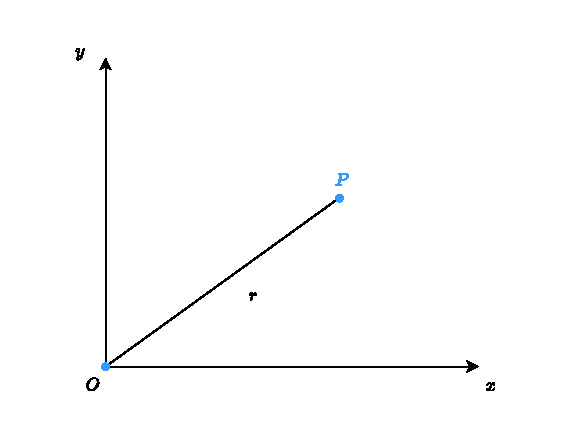
\includegraphics[width=0.6\linewidth]{res/svg/two_dim_IRF.drawio}
\end{figure}
The distance between the origin and $P$ will be:
\begin{equation}
  r = \overline{OP}
\end{equation}
If we send a signal through an electromagnetic wave, it will travel at the speed of light $c$ and reach the point $P$ in a time $t$ given by:
\begin{equation}
  t = \dfrac{r}{c}
\end{equation}
So to synchronize the two clocks, we can use the following procedure:
\begin{enumerate}
  \item Put the clock at distance $r$ already set to $\dfrac{r}{c}$
  \item Send a signal from the origin to the clock and start your clock
  \item When the signal reaches the clock, your clock will read $\dfrac{r}{c}$ and the other one will start from $\dfrac{r}{c}$ aswell
\end{enumerate}
From now on the clocks will be synchronized. This procedure puts us in the perspective that simultaneity is not an absolute concept.
\section{Lorentz transformations}
We need new transformations that work with the principles. We set two IRFs $\irf{R}$ and $\irf{R'}$ in the \textbf{standard configuration}, which means that the $x$ and $x'$ axes coincide and at time $t=0$ we have $O \equiv O'$. The two IRFs are moving with respect to each other with a velocity $v$ along the $x$ axis. Now an event occurs in $P'$, along the $x'$ axis which is at rest with respect to $\irf{R'}$, and we want to find the coordinates of the event in $\irf{R}$.
\begin{figure}[H]
  \centering
  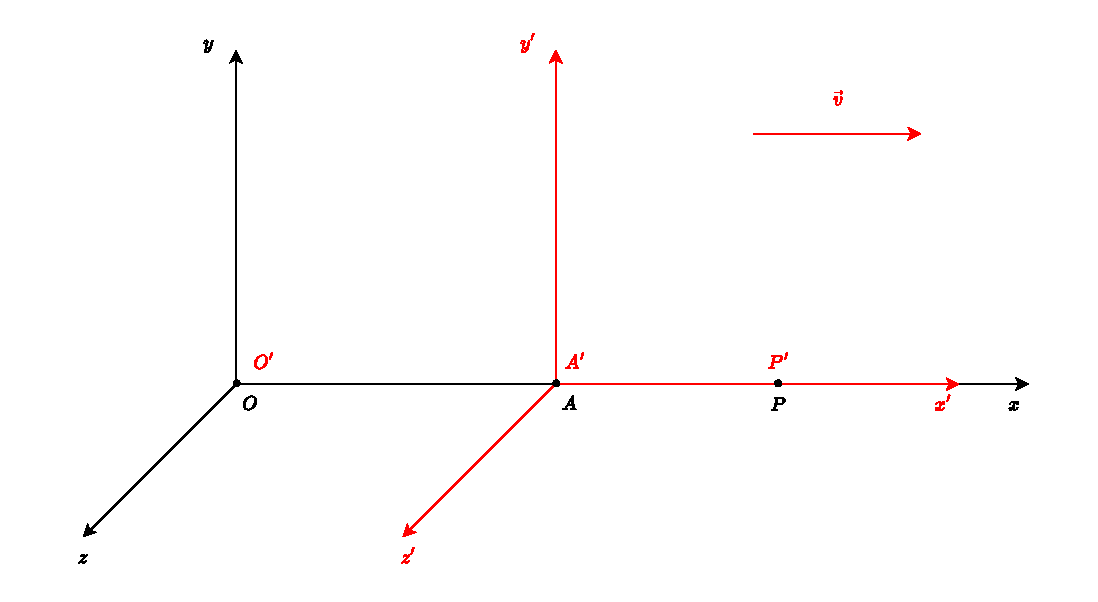
\includegraphics[width=0.6\linewidth]{res/svg/3d_IRF_lorentz.drawio}
  \caption{Moving IRFs}
\end{figure}
If we imagine putting a sort of sign $P$ when the event occurs we might think that it is sufficient to measure the distance $\overline{OP}$, but, in principle, our operational definition of length does not allow us to do that, since we only defined how to measure things at rest with respect to our IRF. Now imagine we mark the points $A'$ (origin of the moving IRF) and $P'$ (event) when the event occurs. The distance we measure will be some sort of proportionality relation depending on the speed of the IRF. We can write:
\begin{equation}
  \overline{A'P'} = \gamma (v)\overline{AP}
\end{equation}
And so:
\begin{equation}
  \overline{OP} = \overline{OA} + \overline{AP} = \overline{OA} + \dfrac{\overline{A'P'}}{\gamma (v)}
\end{equation}
We can also write:
\begin{equation}
  \overline{OA} = vt
\end{equation}
And so:
\begin{equation}
  \overline{OP} = vt + \dfrac{\overline{A'P'}}{\gamma (v)}
\end{equation}
This makes sense since $\gamma (v)$ will be equal to 1 when $v=0$ and so the distance in the second IRF will be equal to the distance we measure in the original one. We can also write:
\begin{equation}
  x = vt + \dfrac{x'}{\gamma(v)} \implies x' = \gamma(v)(x - vt)
\end{equation}
If $\gamma(v)$ were equal to 1, we would have the Galilean transformations. Doing the same reasoning in the other IRF we can find that:
\begin{equation}
 x = \gamma(-v)(x' + vt')
\end{equation}
But since there is no reason for gamma to change if we simply change the direction of the velocity $\gamma(-v) = \gamma(v)$, thus we have:
\begin{equation}
  \begin{split}
    &x = \gamma(v)(x' + vt') = \gamma(v)(\gamma(v)(x - vt) + vt') \\[8pt]
    &\dfrac{x}{\gamma(v)} = \gamma(v)x - \gamma(v)vt + vt' \\[8pt]
    &\underbrace{\dfrac{1}{v}\sqbr{\dfrac{1}{\gamma(v)}- \gamma(v)}}_{\nu(v)}x = t' - \gamma(v)t \\[8pt]
    &\nu(v)x + \gamma(v)t = t'
  \end{split}
\end{equation}
We found that:
\begin{equation} \label{e:lt_start}
  \begin{cases}
    x' = \gamma(v)(x - vt) \\[8pt]
    t' = \nu(v)x + \gamma(v)t \\[8pt]
    y'=y \\[8pt]
    z'=z
  \end{cases}
\end{equation}
We are done if we find the form of $\gamma(v)$. Let's use the fact that light travels at the same speed in both IRFs. Imagine sending a signal between two points at distance $\norm{\vec{r}}$. We have:
\begin{itemize}
  \item Event 1: S emits a signal at $t=t_1$. $E_1 = E_1(x_1, y_1, z_1, t_1)$
  \item Event 2: R receives the signal at $t=t_2$. $E_2 = E_2(x_2, y_2, z_2, t_2)$
\end{itemize}
The distances between the components of the positions of the events are:
\begin{equation}
  \begin{split}
    \Delta x = x_2 - x_1 \\[8pt]
    \Delta y = y_2 - y_1 \\[8pt]
    \Delta z = z_2 - z_1
  \end{split}
\end{equation}
And so the distance between $R$ and $S$ is:
\begin{equation}
  \norm{\Delta \vec{r}} = \sqrt{\Delta x^2 + \Delta y^2 + \Delta z^2}
\end{equation}
Since the signal travels at the speed of light, we have:
\begin{equation}
  \begin{split}
    &\Delta t = \dfrac{\norm{\vec{r}}}{c} = \dfrac{1}{c}\sqrt{\Delta x^2 + \Delta y^2 + \Delta z^2} \\[8pt]
    &\Delta t^2 = \dfrac{1}{c^2}\brackets{\Delta x^2 + \Delta y^2 + \Delta z^2} \\[8pt]
    &\underbrace{c^2\Delta t^2 - \Delta x^2 + \Delta y^2 + \Delta z^2}_{\Delta s^2} = 0\\[8pt]
  \end{split}
\end{equation}
In the second IRF we must have that:
\begin{equation}
  \dfrac{\norm{\Delta \vec{r}'}}{\Delta t'} = c
\end{equation}
And so, when the event occurs:
\begin{equation}
  \Delta s'^2 = \Delta s^2 = 0
\end{equation}
They are both zero since the two events are connected by a light signal. In general (except for light emission/ absorption events) the speed of the signal is not equal to $c$. We can write:
\begin{equation}
  \Delta s^2 = c^2\Delta t^2 - \Delta x^2 - \Delta y^2 - \Delta z^2 \neq 0
\end{equation}
Since the equations of transformation \eqref{e:lt_start} are linear and homogeneous, we know that the two $\Delta^2$s are proportional:
\begin{equation}
  \Delta s'^2 = \alpha \Delta s^2
\end{equation}
But since the events are arbitrary we can set only $\Delta z \neq 0$, but we also remember that $\Delta z = \Delta z'$ and so the only possible value of $\alpha$ is 1. Thus, we have:
\begin{equation}
  \Delta s'^2 = \Delta s^2
\end{equation}
And so $\Delta s$ is invariant under our new transformations. So going back to our original event we remember that the coordinates of $E_1$ are $E_1 = (0,0,0,0)$ and so:
\begin{equation}
  c^2 t^2 - x^2 - \cancel{ y^2} - \cancel{ z^2} = c^2 t'^2 - x'^2 - \cancel{ y'^2} -\cancel{ z'^2}
\end{equation}
Substituting the transformations \eqref{e:lt_start} we have:
\begin{equation}
  c^2 t^2 - x^2 = c^2 \sqbr{\nu(v)x + \gamma(v)t}^2 - \gamma(v)^2(x - vt)^2
\end{equation}
We can group the terms to find something like:
\begin{equation}
  Ax^2 + Bxt + Ct^2 = 0
\end{equation}
But in general this is only true if $A=B=C=0$. Setting $C$ to zero gives:
\begin{equation}
  C = c^2 t^2 - c^2\gamma(v)^2 + \gamma(v)^2v^2 = 0 \implies \gamma(v) = \dfrac{1}{\sqrt{1 - \dfrac{v^2}{c^2}}}
\end{equation}
This is exactly the Lorentz factor we introduced in the previous chapter.
\begin{figure}[H]
  \centering
  \includesvg[width=0.6\linewidth]{res/svg/lorentzfactor}
  \caption{Lorentz factor}
\end{figure}
From now on we call $\gamma(v)$ simply $\gamma$, and we can write the Lorentz transformations as:
\begin{equation} \label{e:lt}
  \begin{cases}
    x' = \gamma(x - vt) \\[8pt]
    y'=y \\[8pt]
    z'=z \\[8pt]
    t' = \gamma\brackets{t - \dfrac{v}{c^2}x} \\[8pt]
  \end{cases}
\end{equation}
These transformations are actually restricted to the motion along the $x$ axis, but we can easily extend them to the other axes by simply rotating the system as we will soon show. Here are some comments about these transformations:
\begin{itemize}
  \item $\gamma$ is always real and greater than 1 since $v<c$ always
  \item If $v \ll c$ we have $\gamma \approx 1$, and so we have the Galilean transformations
  \item If $v \approx c$ we have $\gamma \rightarrow \infty$
  \item If the two IRFs were not in the standard configuration, then the Lorentz transformations would still be linear but not homogeneous (we usually put ourselves in the standard configuration to avoid this problem)
  \item Since the Lorentz transformations are a linear system, we can write them in matrix form
\end{itemize}
Let's see what we can say about the last point. If we just take the vector:
\begin{equation}
  \begin{pNiceMatrix}
    x'\\[8pt]
    y'\\[8pt]
    z'\\[8pt]
    t'\\
  \end{pNiceMatrix}
\end{equation}
Then we have that the linear system \eqref{e:lt} is equivalent to:
\begin{equation}
  \begin{pNiceMatrix}
    x' \\[8pt]
    y' \\[8pt]
    z' \\[8pt]
    t' \\
  \end{pNiceMatrix}
  =
  \begin{pNiceMatrix}[columns-width=auto]
    \gamma & 0 & 0 & -\gamma v \\[8pt]
    0 & 1 & 0 & 0 \\[8pt]
    0 & 0 & 1 & 0 \\[8pt]
    -\gamma \dfrac{v}{c^2} & 0 & 0 & \gamma \\
  \end{pNiceMatrix}
  \begin{pNiceMatrix}
    x \\[8pt]
    y \\[8pt]
    z \\[8pt]
    t \\
  \end{pNiceMatrix}
\end{equation}
But this is rather ugly. In order to make this more elegant we do not use time, but $ct$ so that we have all lengths inside the vector. We then define the vector $x^{\mu}$:
\begin{equation}
  x^0 = ct, \quad x^1 = x, \quad x^2 = y, \quad x^3 = z
\end{equation}
We also define:
\begin{equation}
  \beta \defineeq \dfrac{v}{c}
\end{equation}
And so Lorentz transformations become:
\begin{equation}
  \begin{pNiceMatrix}
    x'^0 \\[8pt]
    x'^1 \\[8pt]
    x'^2 \\[8pt]
    x'^3 \\
  \end{pNiceMatrix}
  =
  \begin{pNiceMatrix}[columns-width=auto]
    \gamma & -\gamma \beta & 0 & 0 \\[8pt]
    -\gamma \beta & \gamma & 0 & 0 \\[8pt]
    0 & 0 & 1 & 0 \\[8pt]
    0 & 0 & 0 & 1 \\
  \end{pNiceMatrix}
  \begin{pNiceMatrix}
    x^0 \\[8pt]
    x^1 \\[8pt]
    x^2 \\[8pt]
    x^3 \\
  \end{pNiceMatrix}
\end{equation}
We define this matrix as the \textbf{Lorentz matrix} $\lm$:
\begin{equation}
  \lm \defineeq
  \begin{pNiceMatrix}[columns-width=auto]
    \gamma & -\gamma \beta & 0 & 0 \\[8pt]
    -\gamma \beta & \gamma & 0 & 0 \\[8pt]
    0 & 0 & 1 & 0 \\[8pt]
    0 & 0 & 0 & 1 \\
  \end{pNiceMatrix}
\end{equation}
\subsection{Composition of boosts}
If we have three IRFs $\irf{R}$, $\irf{R'}$ and $\irf{R''}$ such that $\irf{R'}$ moves with speed $v$ with respect to $\irf{R}$ and $\irf{R''}$ moves with speed $v'$ with respect to $\irf{R'}$. The two speeds are parallel, and we want to find at what speed $\irf{R''}$ moves with speed $v''$ with respect to $\irf{R}$. Obviously this will not just be:
\begin{equation}
  v'' \neq v' + v
\end{equation}
But, by applying the Lorentz transformations two time we get:
\begin{equation}
  v'' = \dfrac{v + v'}{1 + \dfrac{vv'}{c^2}}
\end{equation}
And so those notations are equivalent:
\begin{equation}
  \begin{split}
    &\irf{R} \xrightarrow{\lm(v)} \irf{R'} \xrightarrow{\lm(v')} \irf{R''}\\[8pt]
    &\irf{R} \overset{\lm(v'')}{\xrightarrow{\makebox[2.25cm]{}}} \irf{R''}
  \end{split}
\end{equation}
If we had a boost that isn't parallel to an axis we can just rotate the axes and so the transformation will become:
\begin{equation}
  \irf{R} \xrightarrow{R\lm} \irf{R'}
\end{equation}
The rotation + transformation notation used above is called \textbf{Thomas notation}. Clearly, the matrix $R$ represents the rotation matrix and the matrix $\lm$ still represents the Lorentz transformation. The most general homogeneous Lorentz transformation is then:
\begin{equation}
  R\lm_0
\end{equation}
\subsection{Inverse Lorentz transformations}
Now we can ask ourselves what the inverse of a Lorentz transformation is. We have two ways to determine this. The first is just to write down the equations, invert them and write the inverse matrix $\invlm$:
\begin{equation}
  \begin{cases}
    x' = \gamma(x - vt)\\[8pt]
    y'=y \\[8pt]
    z'=z \\[8pt]
    t' = \gamma\brackets{t - \dfrac{v}{c^2}x} \\[8pt]
  \end{cases}
  \xrightarrow{\text{invert}} \quad
  \begin{cases}
    x = \gamma(x' + vt') \\[8pt]
    y = y' \\[8pt]
    z = z' \\[8pt]
    t = \gamma\brackets{t' + \dfrac{v}{c^2}x'} \\[8pt]
  \end{cases}
\end{equation}
This is a bit long but not difficult.\\
\STOP Otherwise, we can just observe that the matrix $\lm$ can be easily inverted since the $2 \by 2$ block on the bottom right is just the identity matrix. The other block which contains $\gamma$ and $\beta$ can be inverted using the $2 \by 2$ matrix inversion rule. First define the submatrix:
\begin{equation}
  \lm_{2 \by 2} = \begin{pNiceMatrix}[columns-width=auto]
    \gamma & -\gamma \beta \\[8pt]
    -\gamma \beta & \gamma \\[8pt]
  \end{pNiceMatrix}
\end{equation}
Then find the inverse:
\begin{equation}
  \invlm_{2 \by 2} = \dfrac{1}{\det(\lm_{2x2})}\begin{pNiceMatrix}[columns-width=auto]
    \gamma & \gamma \beta \\[8pt]
    \gamma \beta & \gamma \\[8pt]
  \end{pNiceMatrix}
\end{equation}
But the determinant of the submatrix is just:
\begin{equation}
  \det(\lm_{2x2}) = \gamma^2 - \beta^2\gamma^2 = \gamma^2 \bbrackets{\underbrace{1 - \dfrac{v^2}{c^2}}_{1/\gamma^2}} = \cancel{ \gamma^2} \dfrac{1}{\cancel{\gamma^2}} = 1
\end{equation}
And so the inverse Lorentz matrix is:
\begin{equation}
  \invlm =
  \begin{pNiceMatrix}[columns-width=auto]
    \gamma & \gamma \beta & 0 & 0 \\[8pt]
    \gamma \beta & \gamma & 0 & 0 \\[8pt]
    0 & 0 & 1 & 0 \\[8pt]
    0 & 0 & 0 & 1 \\
  \end{pNiceMatrix}
\end{equation}
Which is equivalent to what we got by inverting the system.\\ (End of optional material)
\subsection{Vector form of Lorentz transformations}
For two IRFs in standard configuration we have that the unit vectors are the same:
\begin{equation}
  \begin{split}
    \hat{u}_{x} = \hat{u}_{x'}\\[8pt]
    \hat{u}_{y} = \hat{u}_{y'}\\[8pt]
    \hat{u}_{z} = \hat{u}_{z'}
  \end{split}
\end{equation}
We could represent Galilean transformations as a vector equation:
\begin{equation} \label{e:vector_galilean}
  \vec{r}' = \vec{r} - \vec{v}t
\end{equation}
Where the velocity is:
\begin{equation}
  \vec{v} =
  \begin{pNiceMatrix}
    v \\[8pt] 0 \\[8pt] 0
  \end{pNiceMatrix}
\end{equation}
What about Lorentz transformations? If we eplicitly write the equations we have:
\begin{equation}
  \vec{r}' = \gamma(x-vt)\hat{u}_{x} + y\hat{u}_{y} + z\hat{u}_{z} = \gamma x \hat{u}_{x} - vt\hat{u}_{x} + y\hat{u}_{y} + z\hat{u}_{z}
\end{equation}
If we add and subtract the $x$ component of the position vector we can write Lorentz transformations similarly to \eqref{e:vector_galilean}:
\begin{equation}
  \begin{split}
    \vec{r}' &= \gamma x \hat{u}_{x} - vt\hat{u}_{x} + y\hat{u}_{y} + z\hat{u}_{z} + x \hat{u}_{x} - x \hat{u}_{x}\\[8pt]
    \begin{pNiceMatrix}
      x' \\[8pt] y' \\[8pt] z'
    \end{pNiceMatrix}
    &= \begin{pNiceMatrix}
      x \\[8pt] y \\[8pt] z
    \end{pNiceMatrix}
    + \begin{pNiceMatrix}
      \brackets{\gamma -1}x + \gamma vt \\[8pt] 0 \\[8pt] 0
    \end{pNiceMatrix}
  \end{split}
\end{equation}
But this is not a really nice form. We can rewrite the unit vector and the $x$ component of $\vec{r}$ as:
\begin{equation}
  \begin{split}
    &\hat{u}_{x} = \dfrac{\vec{v}}{v} \\[8pt]
    &x = \vec{r} \cdot \hat{u}_{x} = \dfrac{\vec{r} \cdot \vec{v}}{v}
  \end{split}
\end{equation}
And so we have:
\begin{equation}
  \begin{split}
    \brackets{\gamma -1}x\hat{u}_{x} + \gamma vt\hat{u}_{x} &= \brackets{\gamma -1}\dfrac{\vec{r} \cdot \vec{v}}{v} \dfrac{\vec{v}}{v} + \gamma \cancel{v}t \dfrac{\vec{v}}{\cancel{v}} = \\[8pt]
    & = \vec{v} \sqbr{\brackets{\gamma -1}\dfrac{\vec{r} \cdot \vec{v}}{v^2} + \gamma t}
  \end{split}
\end{equation}
And so we can write Lorentz transformations as:
\begin{equation}
  \begin{cases}
    \vec{r}' = \vec{r} + \vec{v} \sqbr{\brackets{\gamma - 1} \dfrac{\vec{r} \cdot \vec{v}}{v^2} + \gamma t} \\[8pt]
    t' = \gamma \brackets{t - \dfrac{\vec{r} \cdot \vec{v}}{c^2}}
  \end{cases}
\end{equation}
The advantage of this form is that those equations are true for any boost in any direction.
\subsection{Time order}
These new transformations implicitly imply that there could be some ``weird'' stuff happening to the order of events. Since time and thus simultaneity depend on position and velocity we can ask ourselves if it is possible to find a couple of IRFs in motion with respect to each other such that an event $E_A(x_A,y_A,z_A,t_A)$ happens before a second event $E_B(x_B,y_B,z_B,t_B)$ in one IRF, but $E_B$ happens before $E_A$ in the other.\\
Let's start from two events only separated along the $x$ component. Defining the time interval $\Delta t = t_B - t_A$ we want that:
\begin{equation}
  \begin{split}
    \Delta t > 0 \quad \text{in} \irf{R} \\[8pt]
    \Delta t' < 0 \quad \text{in} \irf{R}'
  \end{split}
\end{equation}
We can just apply Lorentz transformations in the second equation and see what we find. Since they are linear we can substite $\Delta x$ instead of $x$ and $\Delta t$ instead of $t$, but in principle we should substite every single term and then group. We have:
\begin{equation}
  \Delta t' = \gamma \brackets{\Delta t - \dfrac{v}{c^2}\Delta x} < 0 \implies \Delta x > \dfrac{c^2}{v}\Delta t
\end{equation}
For any $v$ we know that $\dfrac{c}{v} > 1$, and so we can find that at least:
\begin{equation}
  \Delta x > c\Delta t
\end{equation}
But $\Delta x = c\Delta t$ is the distance travelled by light in a time interval $\Delta t$, so this means that in order to find a couple of IRFs where the time order of the events is swapped, we must make sure that the events are distant enough to satisfy:
\begin{equation}
  \Delta x > c\Delta t
\end{equation}
It is easy to generalize this condition:
\begin{equation}
  \Delta \norm{\vec{r}} > c\Delta t
\end{equation}
Where $\vec{r}$ is the distance vector between the points where the events take place.\\
This result also means that special relativity \textbf{preserves causality}. If an event is caused by another one there is no way for the signal that connects the two events to travel faster than light, and so we cannot see the time order reversed.
\subsection{Length contraction}
Let's go back to the starting configuration we used to derive Lorentz transformations. We found out that:
\begin{equation}
  \overline{AP} = \dfrac{\overline{A'P'}}{\gamma}
\end{equation}
Let's give a new definition:
\begin{definition}{Proper length}
  The proper length $L_0$ is the length measured in the IRF where the object is stationary.
\end{definition}
And so in our case $\overline{A'P'}$ is the proper length. We can see proper length as the only length that can be directly measured using our definition. We notice that, since $\gamma >1$:
\begin{equation}
  \overline{AP} < \overline{A'P'}
\end{equation}
Thus, proper length is the biggest length measured in any IRF. This result is widely known as \textbf{length contraction}.
\subsection{Time dilation}
We have a similar result for time. Let's imagine an IRF where two events happen in the same point but at different times. In any other IRF in motion with respect to the first one we have:
\begin{equation}
  \Delta t' = \gamma\brackets{\Delta t - \dfrac{v}{c^2}\cancel{\Delta x}} = \gamma \Delta t
\end{equation}
Since $\gamma > 1$ we have that:
\begin{equation}
  \Delta t' > \Delta t
\end{equation}
In this case the time separation between the two events is bigger for the moving observer. This effect is in fact called \textbf{time dilation}. Similarly to what we did with length we can give a new definition:
\begin{definition}{Proper time}
  The proper time $T_0$ is the time interval of the IRF where I measure it with only one clock.
\end{definition}
\subsection{Muons}
To showcase a real example, where the effect of time dilation and length contraction play a crucial role in explaining the phenomenon, we will now talk about \textbf{muons} $\mu$. Muons are a type of elementary particles with these properties:
\begin{itemize}
  \item Charge: $q_{\mu} = -e$
  \item Mass: $m_{\mu} \ll m_{e}$
  \item Proper time decay: $T_0 = \qty{2.2}{\micro\second}$
\end{itemize}
\begin{figure}[H]
  \centering
  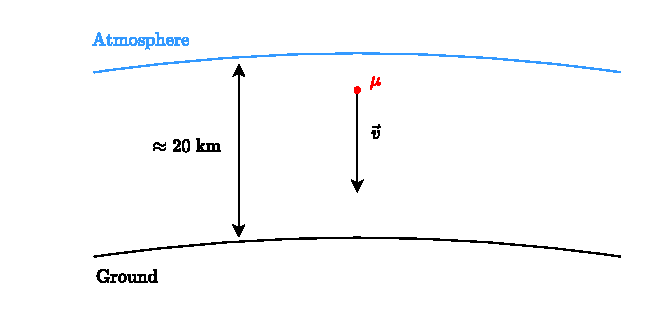
\includegraphics[width=0.8\linewidth]{res/svg/muons_bad.drawio}
  \caption{Muons travelling in Earth's atmosphere}
\end{figure}
Muons are generated by cosmic rays when hitting Earth's atmosphere and, after being generated, they travel at $v \approx 99.89\%\;c$ with a Lorentz factor of $\gamma \approx 30$. Muons were experimentally detected at Earth's surface, but if we apply a classical reasoning, in order to reach the surface of Earth, muons should travel a distance $\Delta x$ in a time less or equal to $T_0$, but this is not the case since $\Delta x \approx \qty{20}{\kilo\meter}$ and so:
\begin{equation}
  \dfrac{\Delta x}{v} \approx \qty{66.7}{\micro\second}
\end{equation}
Instead, applying Einstein's Special Relativity we know that the muon's time is dilated and so:
\begin{equation}
  T_0' = \gamma T_0 = \qty{66}{\micro\second}
\end{equation}
And so this result is compatible with the experimental observations. We can also think that the muon sees Earth travelling with speed $v$ in his direction and so the distance $\Delta x$ will be contracted:
\begin{equation}
  \Delta x' = \dfrac{\Delta x}{\gamma} \approx \qty{666.7}{\meter}
\end{equation}
Thus, the time it would take for the muon to travel this path is:
\begin{equation}
  \dfrac{\Delta x'}{v} \approx \qty{2.23}{\micro\second}
\end{equation}
Again this is coherent with the experimental evidence.
\subsection{Lorentz transformations of the velocities}
In a simple Galilean transformation the velocities are obtained by deriving with respect to time each component of the position:
\begin{equation}
  \begin{cases}
    x' = x - vt \\[8pt]
    y' = y \\[8pt]
    z' = z
  \end{cases} \xrightarrow{\frac{\diff{}}{\diff{t}}}
  \begin{cases}
    u'_x = u_x - v \\[8pt]
    u'_y = u_y \\[8pt]
    u'_z = u_z
  \end{cases}
\end{equation}
But in Lorentz transformation we need to evaluate the derivative of the new coordinates with respect to the new time. Writing Lorentz transformations for an infinitesimal displacement gives:
\begin{equation}
  \begin{cases}
    \diff{x'} = \gamma \brackets{\diff{x} - v \diff{t}} \\[8pt]
    \diff{y'} = \diff{y} \\[8pt]
    \diff{z'} = \diff{z} \\[8pt]
    \diff{t'} = \gamma \brackets{\diff{t} - \dfrac{v}{c^2} \diff{x}}
  \end{cases}
\end{equation}
And so $u'_x$ becomes:
\begin{equation}
  \begin{split}
    u'_x = \dv{x'}{t'} &= \dfrac{\cancel{\gamma} \brackets{\diff{x} - v \diff{t}}}{\cancel{\gamma} \brackets{\diff{t} - \dfrac{v}{c^2} \diff{x}}} =\\[8pt]
    &= \cancel{\dv{t}{t}}\dfrac{\brackets{\dv{x}{t} - v}}{\brackets{1 - \dfrac{v}{c^2} \dv{x}{t}}} = \dfrac{\brackets{u_x - v}}{1 - \dfrac{v u_x}{c^2} }
  \end{split}
\end{equation}
Instead for $u_y$ we have:
\begin{equation}
  \begin{split}
    u'_y = \dv{y'}{t'} &= \dfrac{\diff{y}}{\gamma \brackets{\diff{t} - \dfrac{v}{c^2} \diff{x}}} =\\[8pt]
  &= \dv{y}{t}\dfrac{\sqrt{1-\dfrac{v^2}{c^2}}}{\brackets{1 - \dfrac{v}{c^2} \dv{x}{t}}} = \dfrac{u_y\sqrt{1-\dfrac{v^2}{c^2}}}{1 - \dfrac{v u_x}{c^2}}
  \end{split}
\end{equation}
The same derivation leads to $u'_z$:
\begin{equation}
  u'_z = \dfrac{u_z\sqrt{1-\dfrac{v^2}{c^2}}}{1 - \dfrac{v u_x}{c^2}}
\end{equation}
And so the Lorentz transformation of the velocities for a boost along the x axis are:
\begin{equation}
  \begin{cases}
    u'_x = \dfrac{\brackets{u_x - v}}{1 - \dfrac{v u_x}{c^2}} \\[18pt]
    u'_y = \dfrac{u_y\sqrt{1-\dfrac{v^2}{c^2}}}{1 - \dfrac{v u_x}{c^2}} \\[18pt]
    u'_z = \dfrac{u_z\sqrt{1-\dfrac{v^2}{c^2}}}{1 - \dfrac{v u_x}{c^2}}
  \end{cases}
\end{equation}
If we want to invert the equations and get $u_x, u_y, u_z$ as functions of the new coordinates we simply substitute $v \rightarrow -v$ since the only thing that changes is the direction of $v$:
\begin{equation}
  \begin{cases}
    u_x = \dfrac{\brackets{u'_x + v}}{1 + \dfrac{v u'_x}{c^2}} \\[18pt]
    u_y = \dfrac{u'_y\sqrt{1-\dfrac{v^2}{c^2}}}{1 + \dfrac{v u'_x}{c^2}} \\[18pt]
    u_z = \dfrac{u'_z\sqrt{1-\dfrac{v^2}{c^2}}}{1 + \dfrac{v u'_x}{c^2}}
  \end{cases}
\end{equation}
Now we can see how the magnitude of $u$ changes with a Lorentz transformation. After some calculations it is possible to arrive to:
\begin{equation}
  c^2 - u^2 = \dfrac{c^2\brackets{c^2 - u^{'^2}}\brackets{c^2 - v^2}}{\brackets{c^2 + u'_x v}}
\end{equation}
If we write $u_x$ as:
\begin{equation}
  u_x' = \vec{u}' \cdot \hat{u}_x = \vec{u}' \cdot \dfrac{\vec{v}}{v}
\end{equation}
We have:
\begin{equation}
  c^2 - u^2 = \dfrac{c^2\brackets{c^2 - u^{'^2}}\brackets{c^2 - v^2}}{\brackets{c^2 + \vec{u}'\cdot\vec{v}}}
\end{equation}
This also leads to the result that:
\begin{equation}
  u' < c \iff u < c
\end{equation}
The meaning of this is that, even if an object is moving at speed close to $c$ and another object is thrown from the moving one, the velocity of the thrown item can never be equal or greater to $c$.\\
It is possible to arrive to a vector form of the transformation of velocities. Similarly to what we did to the components we have:
\begin{equation}
  \vec{u}' = \dv{\vec{r}'}{t'}
\end{equation}
After some calculations we arrive to:
\begin{equation}
  \vec{u}' = \dfrac{\dfrac{\vec{u}}{\gamma(v)}+ \vec{v}\sqbr{\dfrac{\vec{u}\cdot\vec{v}}{v^2}\brackets{1-\dfrac{1}{\gamma(v)}}-1}}{1 - \dfrac{\vec{u}\cdot\vec{v}}{c^2}}
\end{equation}
Inverting this equation gives:
\begin{equation}
  \vec{u} = \dfrac{\dfrac{\vec{u}'}{\gamma(v)} - \vec{v}\sqbr{-\dfrac{\vec{u}'\cdot\vec{v}}{v^2}\brackets{1-\dfrac{1}{\gamma(v)}}-1}}{1 + \dfrac{\vec{u}'\cdot\vec{v}}{c^2}}
\end{equation}
Those two formulas are sometimes expressed as the result of a new operation called \textbf{relativistic addition}:
\begin{equation}
  \begin{split}
    \vec{u}' = \vec{v} \oplus \vec{u} \\[8pt]
    \vec{u} = \vec{v} \oplus \vec{u}'
  \end{split}
\end{equation}
Note that this operation is not linear and is not commutative:
\begin{equation}
  \vec{v} \oplus \vec{u} \neq \vec{u} \oplus \vec{v}
\end{equation}
But the magnitude of the results are the same:
\begin{equation}
  \norm{\vec{v} \oplus \vec{u}} = \norm{\vec{u} \oplus \vec{v}}
\end{equation}
Now let's analyse the case where $\vec{v} \perp \vec{u}'$ we have:
\begin{equation}
  \vec{u} = \dfrac{\dfrac{\vec{u}'}{\gamma(v)} - \vec{v}\sqbr{-\dfrac{\cancel{\vec{u}'\cdot\vec{v}}}{v^2}\brackets{1-\dfrac{1}{\gamma(v)}}-1}}{1 + \dfrac{\cancel{\vec{u}'\cdot\vec{v}}}{c^2}} = \dfrac{\vec{u}'}{\gamma (v)} + \vec{v}
\end{equation}
And so for a boost in this configuration:
\begin{figure}[H]
  \centering
  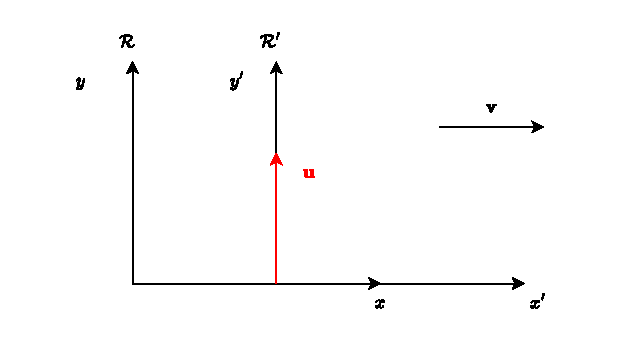
\includegraphics[width=0.6\linewidth]{res/svg/perpendicular_moving.drawio}
\end{figure}
We have that the relativistic addition is just scaled down of a factor $\gamma$ along the $\vec{u}$ vector:
\begin{figure}[H]
  \centering
  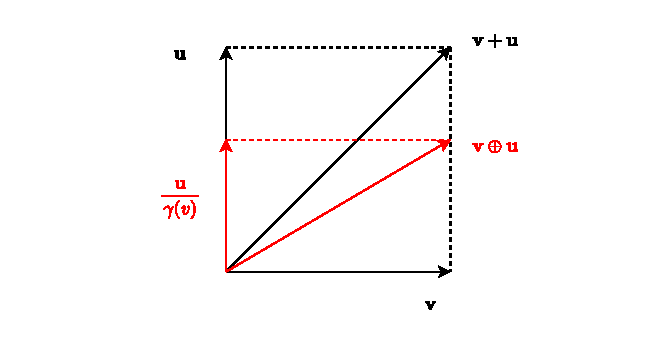
\includegraphics[width=0.8\linewidth]{res/svg/relativistic_addition.drawio}
\end{figure}
\subsection{Lorentz transformation of the $\gamma$ factor}
The Lorentz factor of a moving object changes with respect to the IRF. We have that:
\begin{equation}
  \dfrac{\gamma(u')}{\gamma(u)} = \gamma(v)\brackets{1-\dfrac{\vec{v}\cdot\vec{u}}{c^2}}
\end{equation}
Since this is in vector form it is valid for any boost.
\section{Examples (WIP)}
\section{Doppler effect}
Let us now describe a phenomenon arising from the properties of special relativity, this phenomenon is called \textbf{Relativistic Doppler effect}. First we need to discuss the classical derivation of the Doppler effect.
\begin{figure}[H]
  \centering
  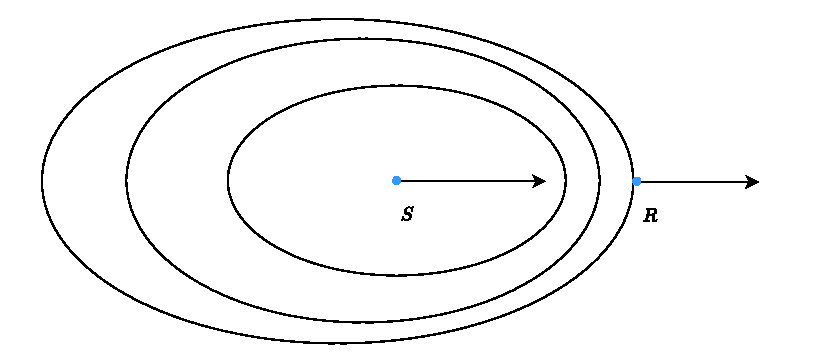
\includegraphics[width=1\linewidth]{res/svg/classical_doppler_diagram.drawio}
\end{figure}
The problem is described with these informations:
\begin{itemize}
  \item A source $S$ generates a signal at time $t=0$
  \item A receiver $R$ receives the signal
  \item The starting distance between the two is $l_0$
  \item Both the receiver and the source are moving in the same direction with, in general, different velocities
\end{itemize}
The fourth assumption is justified since if the source travels in another direction, the only significant component of the velocity that causes the Doppler effect is the component along the line from the source to the receiver.
Now let's start with the discussion.\\
The signal sent by the source reaches the receiver at time $\tau$, but what distance did the signal travel?\\
\begin{figure}[H]
  \centering
  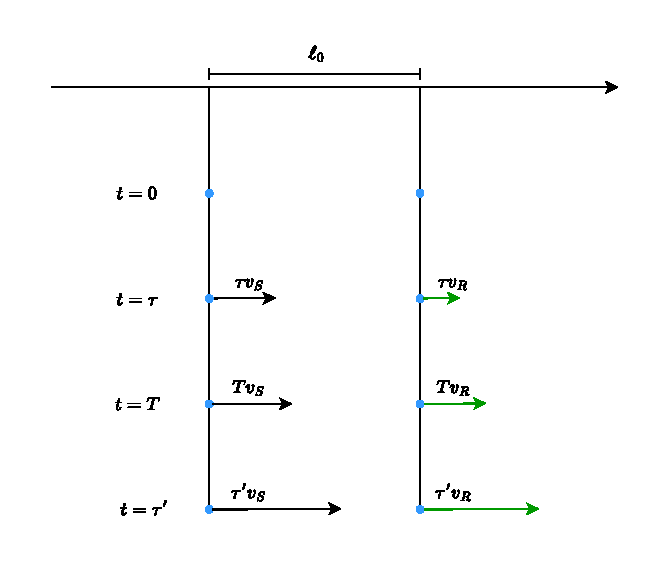
\includegraphics[width=0.8\linewidth]{res/svg/classical_doppler_distances.drawio}
\end{figure}
Since the receiver is moving we need to add the distance travelled by it in the time $\tau$, so:
\begin{equation}
  L_{true} = l_0 + v_{R}\tau
\end{equation}
And so the wave with velocity $v$ travelled $L_{true}$ space in $\tau$ time:
\begin{equation}
  v\tau = l_0 + v_{R}\tau \implies \tau = \dfrac{l_0}{v-v_{R}}
\end{equation}
Now, at time $T$ the source emits another signal, which arrives at the receiver at time $\tau'$, but then the length travelled in the time interval $\tau'-T$ is:
\begin{equation}
  L'_{true} = l_0 - v_{S}T + v_{R}\tau'
\end{equation}
And so:
\begin{equation}
  \begin{split}
    v(\tau'-T) &= l_0 - v_{S}T + v_{R}\tau' \\[8pt]
    \tau'(v-v_{R}) &= l_0 -v_{S}T + vT \\[8pt]
    \tau' &= \dfrac{l_0 +T(v-v_{S})}{v-v_{R}}
  \end{split}
\end{equation}
What is the period between the two signals? We define $T' = \tau' - \tau$ and so:
\begin{equation}
  T' = \dfrac{\cancel{l_0} +T(v-v_{S}) - \cancel{l_0}}{(v-v_{R})} = \dfrac{v-v_{S}}{v-v_{R}}T
\end{equation}
Since the frequency is just the inverse of the period:
\begin{equation}
  \boxed{\nu' = \dfrac{v-v_{R}}{v-v_{S}}\nu'}
\end{equation}
After this we can start to describe the relativistic version of this problem. The differences between the two situations are essentially three:
\begin{itemize}
  \item The signal does not propagate in a medium
  \item The relative velocity, in general, is not moving along the direction $S-R$, but is a generic $\vec{v}$
\end{itemize}
Let's choose two IRFs:
\begin{itemize}
  \item $\irf{R}$ is such that $R$ is stationary
  \item $\irf{R'}$ is such that $S$ is stationary
\end{itemize}
The first event is:
\begin{quotation}
  Event A: $S$ emits light in $O \equiv O'$ at time $t = t' = 0$
\end{quotation}
Now we state that phase is Lorentz invariant (this will be more clear later), thus both observers will agree on seeing when the EM fields are at a peak:
\begin{equation}
  k_{R}r-\omega_{R} t = k_{S}r' - \omega_{S} t'
\end{equation}
Let's group the angular frequencies, knowing that $\dfrac{k}{\omega} = \dfrac{2\pi}{\lambda}\dfrac{1}{2\pi\nu} = \dfrac{1}{c}$ we get:
\begin{equation}
  \omega_{R}\brackets{t-\dfrac{r}{c}} = \omega_{S}\brackets{t'-\dfrac{r'}{c}}
\end{equation}
Now let's picture the situation when the receiver registers the signal:
\begin{quotation}
  Event B: $R$ receives the signal
\end{quotation}
\begin{figure}[H]
  \centering
  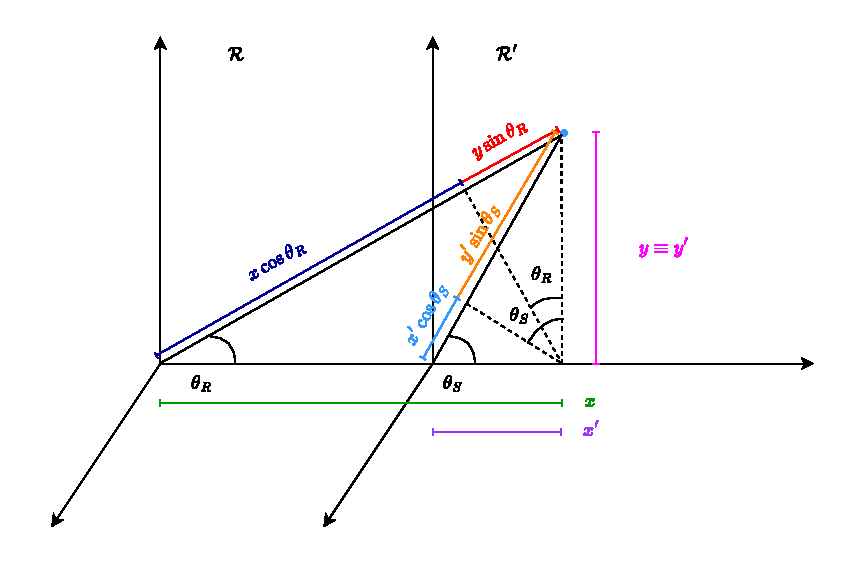
\includegraphics[width=0.8\linewidth]{res/svg/Doppler_geometry.drawio}
\end{figure}
So the modulus of $\vec{r}$ and $\vec{r}'$ are:
\begin{equation}
  \begin{split}
    &r = x\cos\theta_R + y\sin\theta_R \\[8pt]
    &r' = x'\cos\theta_S + y'\sin\theta_S
  \end{split}
\end{equation}
And so, since the two phases must be equal:
\begin{equation}
  \omega_{R}\sqbr{t-\dfrac{1}{c}\brackets{x\cos\theta_R + y\sin\theta_R}} = \omega_{S}\sqbr{t'-\dfrac{1}{c}\brackets{x'\cos\theta_S + y'\sin\theta_S}}
\end{equation}
Now we substite what we know from the Lorentz transformation of this system:
\begin{equation}
  \begin{cases}
    x' = \gamma(x - vt) \\[8pt]
    y' = y \\[8pt]
    t' = \gamma\brackets{t - \dfrac{v}{c^2}x}
  \end{cases}
\end{equation}
Thus the equation will be:
\begin{equation}
  \omega_{R}\sqbr{t-\dfrac{1}{c}\brackets{x\cos\theta_R + y\sin\theta_R}} = \omega_{S}\sqbr{\gamma\brackets{t - \dfrac{v}{c^2}x} - \dfrac{1}{c}\brackets{\gamma(x - vt)\cos\theta_S + y\sin\theta_S}}
\end{equation}
This must be true for all $x,y,t$ and so every coefficient must coincide.\\
For $t$ (1):
\begin{equation}
  \omega_R  = \omega_S \gamma\brackets{1 + \dfrac{v}{c}\cos \theta_S}
\end{equation}
For $x$ (2):
\begin{equation}
  \begin{split}
    \cancel{-}\dfrac{\omega_R}{\cancel{c}}\cos \theta_R &= \cancel{-}\omega_S \dfrac{\gamma}{\cancel{c}}\brackets{\dfrac{v}{c} + \cos \theta_S}\\[8pt]
    \cos \theta_R  &= \dfrac{\omega_S}{\omega_R} \gamma \brackets{\dfrac{v}{c} + \cos \theta_S} =\\[8pt]
    &\overset{(1)}{=} \dfrac{1}{\cancel{\gamma}\brackets{1 + \dfrac{v}{c}\cos \theta_S}} \cancel{\gamma} \brackets{\dfrac{v}{c} + \cos \theta_S} =\\[8pt]
    &= \dfrac{\dfrac{v}{c} + \cos \theta_S}{1 + \dfrac{v}{c}\cos \theta_S}
  \end{split}
\end{equation}
For $y$ (3):
\begin{equation}
  \begin{split}
    \cancel{-}\dfrac{\omega_R}{\cancel{c}}\sin \theta_R &= \cancel{-}\omega_S \dfrac{\gamma}\sin \theta_S\\[8pt]
    \sin \theta_R &= \dfrac{\omega_S}{\omega_R}\sin \theta_S = \\[8pt]
    &\overset{(1)}{=} \dfrac{1}{\gamma\brackets{1 + \dfrac{v}{c}\cos \theta_S}}\sin \theta_S = \\[8pt]
    &= \dfrac{\sqrt{1-\dfrac{v^2}{c^2}}}{1 + \dfrac{v}{c}\cos \theta_S}\sin \theta_S
  \end{split}
\end{equation}
And so, from (1) and (2) we can evaluate $\tan \theta_R$:
\begin{equation}
  \begin{split}
    \tan \theta_R = \dfrac{\sin \theta_R}{\cos \theta_R} &= \dfrac{\dfrac{\sqrt{1-\dfrac{v^2}{c^2}}}{1 + \dfrac{v}{c}\cos \theta_S}\sin \theta_S}{\dfrac{\dfrac{v}{c} + \cos \theta_S}{1 + \dfrac{v}{c}\cos \theta_S}} = \\[8pt]
    &= \dfrac{\sqrt{1-\dfrac{v^2}{c^2}}\sin \theta_S}{\cos \theta_S + \dfrac{v}{c}} = \\[8pt]
    &= \dfrac{c\sqrt{1-\dfrac{v^2}{c^2}}\sin \theta_S}{c\cos \theta_S + v}
  \end{split}
\end{equation}
Let's compare this to what we got for the transformation of the velocities:
\begin{equation}
  \tan \theta = \dfrac{u'\sin \theta'}{u'\cos \theta' + u}\dfrac{1}{\gamma}
\end{equation}
This is the same formula with:
\begin{equation}
  \begin{split}
    &u' = c \\[8pt]
    &\theta = \theta_R \\[8pt]
    &\theta' = \theta_S
  \end{split}
\end{equation}
If we write down both the relativistic and the classical Doppler effect we have:
\begin{equation}
  \begin{split}
    \omega_R  = \omega_S \gamma\brackets{1 + \dfrac{v}{c}\cos \theta_S} \\[8pt]
    \omega_R = \omega_S \dfrac{v - v_R}{v - v_S}
  \end{split}
\end{equation}
The two phenomenona cannot be really compared since the EM waves which generate the relativistic version of the Doppler effect do not require a medium to travel, but if we see that $-v \cos \theta_S$ is actually the tangential component of $v$ in the IRF $\irf{R}'$, thus it is similar to $v_R$ and we can write:
\begin{equation}
  \omega_R  = \omega_S \gamma\dfrac{c - v_R}{c}
\end{equation}
This relation is similar to the classical one with two exceptions:
\begin{enumerate}
  \item $v_S = 0$ in the relativistic case. The only quantity that matters is the relative velocity between the source and the receiver
  \item The Lorentz factor $\gamma$ is present
\end{enumerate}
This leads to a new situation which was not present in the classical case. If we consider a source in tangential motion there is no classical Doppler effect since the distance is kept constant, but in the relativistic case we have a transverse Doppler effect:
\begin{equation}
  \theta_S = \dfrac{\pi}{2} \implies \cos \theta_S = 0
\end{equation}
And so:
\begin{equation}
  \omega_R  = \omega_S \gamma \implies \omega_R  > \omega_S
\end{equation}
This effect is called \textbf{Blue shift} since the light that arrives at the receiver has a higher frequency, which results in a smaller wavelength and so, for example, a red beam of light will be shifted towards blue.\\
Similarly, if a source is moving away from the observer we have:
\begin{equation}
  \theta_S = \pi \implies \cos \theta_S = -1
\end{equation}
Which leads to:
\begin{equation}
  \begin{split}
    \omega_R  &= \omega_S \gamma\brackets{1 - \dfrac{v}{c}} = \\[8pt]
    &= \omega_S \dfrac{1 - \dfrac{v}{c}}{\sqrt{1 - \dfrac{v^2}{c^2}}} = \\[8pt]
    &= \omega_S \sqrt{\dfrac{\brackets{1 - \dfrac{v}{c}}^{\cancel{2}}}{\cancel{\brackets{1 - \dfrac{v}{c}}}\brackets{1 + \dfrac{v}{c}}}} = \\[8pt]
    &= \omega_S \sqrt{\dfrac{\brackets{1 - \dfrac{v}{c}}}{\brackets{1 + \dfrac{v}{c}}}}
  \end{split}
\end{equation}
This means that $\omega_R < \omega_S$ and so we have a higher wavelength. This phenomenon is called \textbf{Red shift}.
\begin{figure}[H]
    \begin{minipage}{0.5\textwidth}
     \centering
     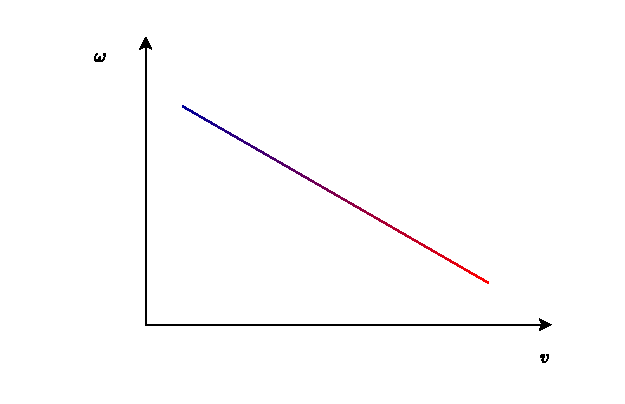
\includegraphics[width=1\linewidth]{res/svg/Doppler_redshift.drawio}
     \caption{Red shift}
   \end{minipage}\hfill
   \begin{minipage}{0.5\textwidth}
     \centering
     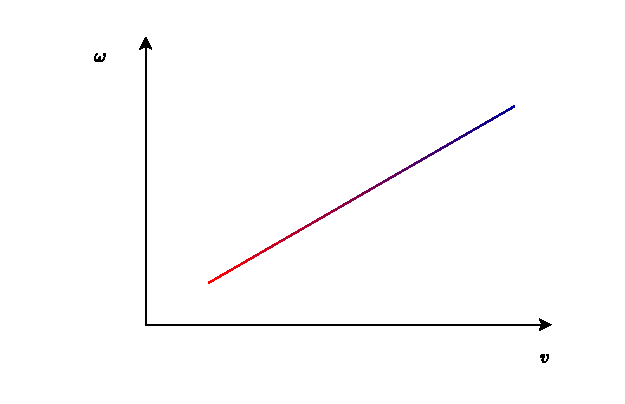
\includegraphics[width=1\linewidth]{res/svg/Doppler_blueshift.drawio}
     \caption{Blue shift}
   \end{minipage}
\end{figure}
\STOP We can check that the coefficients of $\omega_R = K\omega_S$ in the cases of rotations of $n\dfrac{\pi}{2}$ are related to the eigenvalues associated to the Lorentz matrix.\\
We know that $1$ will be an eigenvalue because of the 2x2 block on the bottom right of the Lorentz matrix, so we just need the eigenvalues of the $2 \by 2$ block on the top left:
\begin{equation}
  \lm_{2 \by 2} = \begin{pNiceMatrix}[columns-width=auto]
    \gamma & -\gamma \beta \\[8pt]
    -\gamma \beta & \gamma \\[8pt]
  \end{pNiceMatrix}
\end{equation}
We find $\lambda_1, \lambda_2$ by the usual method:
\begin{equation}
  p(\lambda) = \det(\lm_{2 \by 2} - \lambda \mathbb{I}) = \brackets{\gamma - \lambda}^2 - \gamma^2\beta^2 = \gamma^2 -2\gamma\lambda +\lambda^2 - \gamma^2\beta^2
\end{equation}
Finding the eigenvalues means:
\begin{equation}
  p(\lambda) = 0 \implies \lambda^2 -2\cancel{\gamma}\lambda + \gamma^{\cancel{2}}- \gamma^{\cancel{2}}\beta^2 = 0 \\[8pt]
\end{equation}
\begin{equation}
  \begin{split}
    &\dfrac{1}{\gamma}\lambda^2 -2\lambda +\gamma \brackets{1- \beta^2} = 0 \\[8pt]
    &\dfrac{1}{\gamma}\lambda^2 -2\lambda + \dfrac{1}{\sqrt{1-\beta^2}} \brackets{1- \beta^2} = 0 \\[8pt]
    &\dfrac{1}{\gamma}\lambda^2 -2\lambda + \sqrt{\dfrac{\brackets{1- \beta^2}^2}{1-\beta^2}}  = 0 \\[8pt]
    &\sqrt{1- \beta^2}\lambda^2 -2\lambda + \sqrt{1- \beta^2}  = 0 \\[8pt]
  \end{split}
\end{equation}
And so the roots are easily found by:
\begin{equation}
  \begin{split}
    \lambda_{1,2} &= \dfrac{2\pm\sqrt{4 - 4\brackets{1-\beta^2}}}{2} =\\[8pt]
    & = \dfrac{2\pm\sqrt{\cancel{4} - \cancel{4} +4\beta^2}}{2} =\\[8pt]
    & = \dfrac{2 \pm 2\beta}{2} = 1 \pm \beta
  \end{split}
\end{equation}
Thus the set of all the eigenvalue of $\lm$ is:
\begin{equation}
  \mathrm{spec}(\lm) = \{1, 1 \pm \beta\}
\end{equation}
Notice that for the various cases of rotations of $\dfrac{n\pi}{2}$ we have:
\begin{table}[H]
  \centering
  \begin{tabular}{lc}
    $\omega_R = \gamma \brackets{1-\beta} \omega_S$ & (for $n$ = 1) \\[8pt]
    $\omega_R = \gamma \omega_S$ & (for $n$ = 2) \\[8pt]
    $\omega_R = \gamma \brackets{1+\beta} \omega_S$ & (for $n$ = 3) \\[8pt]
    $\omega_R = \gamma \omega_S$ & (for $n$ = 4) \\[8pt]
  \end{tabular}
\end{table}
(End of optional material)
\begin{exercise}{TO DO}

\end{exercise}
